\newpage
\section[Фигура 5]{Фигура 5}

Строим круги, используя примитивы \textbf{Inkscape}.
Последовательно применяем операции
\textit{\textbf{Duplicate, Exclusion, Division}}, заливка, перемещение, выравнивание фигур.

\begin{figure}[H]
    \begin{minipage}[h]{0.47\linewidth}
        \center{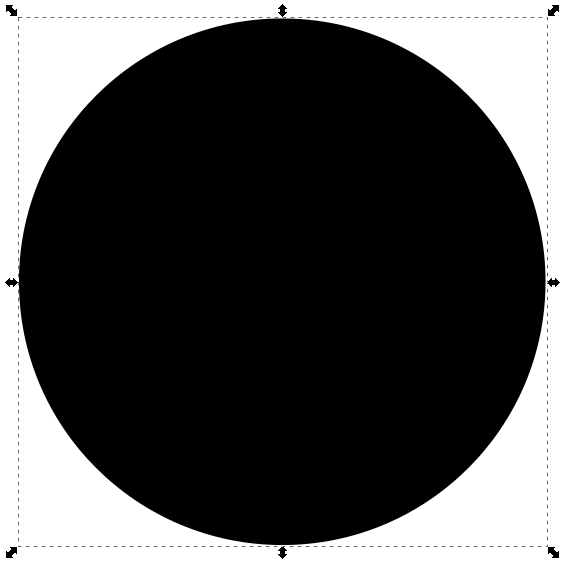
\includegraphics[width=1\linewidth]{5_1_create.png}}\\
        Создание фигур
    \end{minipage}
    \hfill
    \begin{minipage}[h]{0.47\linewidth}
        \center{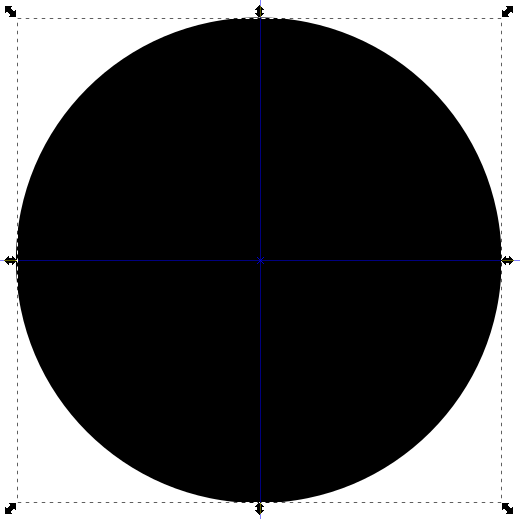
\includegraphics[width=1\linewidth]{5_2_guidelines.png}}\\
        Добавление вспомагательных линий
    \end{minipage}
    \vfill
    \vspace*{1cm}
    \begin{minipage}[h]{0.47\linewidth}
        \center{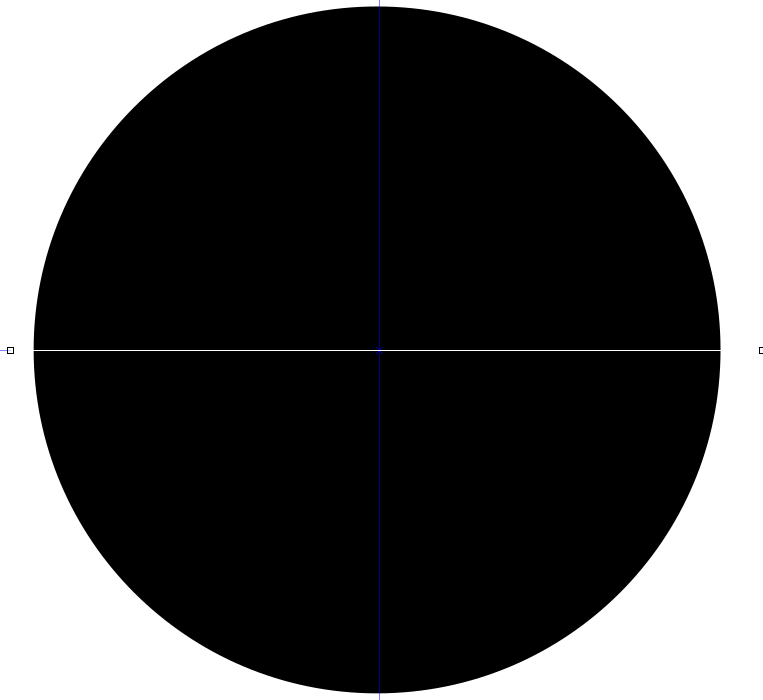
\includegraphics[width=1\linewidth]{5_3_divide_line.png}}\\
        Создание линии разделения
    \end{minipage}
    \hfill
    \begin{minipage}[h]{0.47\linewidth}
        \center{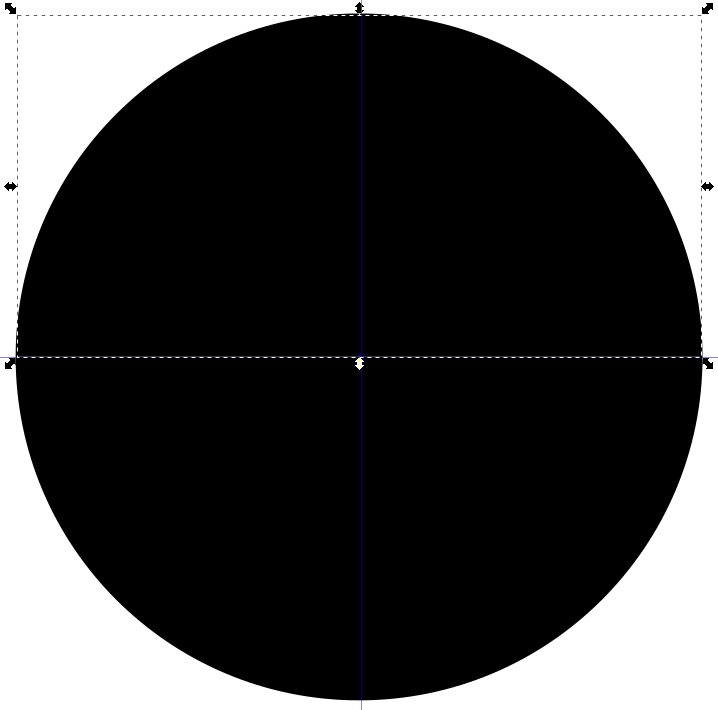
\includegraphics[width=1\linewidth]{5_4_division.png}}\\
        Разделение фигуры
    \end{minipage}
\end{figure}
\newpage
\begin{figure}[H]
    \begin{minipage}[h]{0.47\linewidth}
        \center{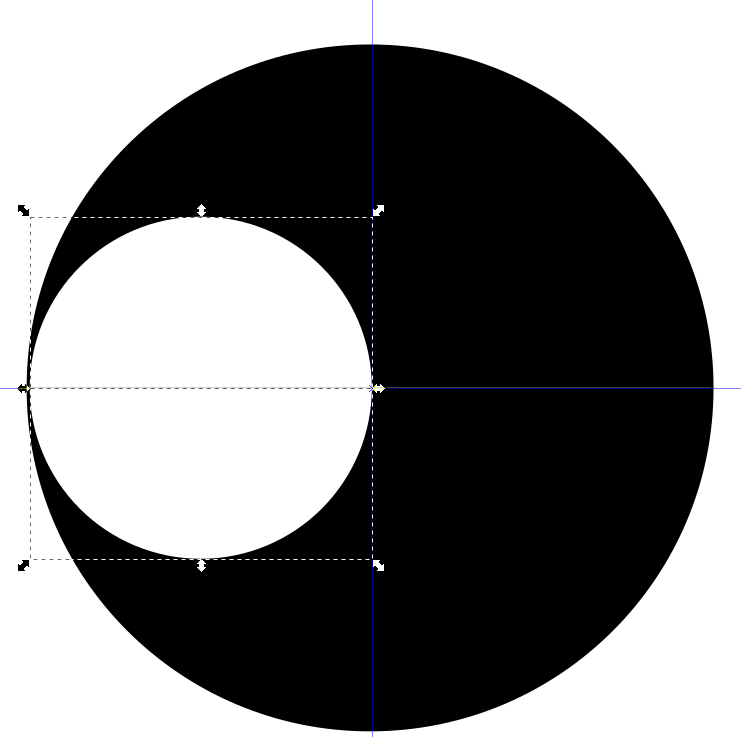
\includegraphics[width=1\linewidth]{5_5_duplicate.png}}\\
        Дублирование фигуры, изменение размера и цвета заливки
    \end{minipage}
    \hfill
    \begin{minipage}[h]{0.47\linewidth}
        \center{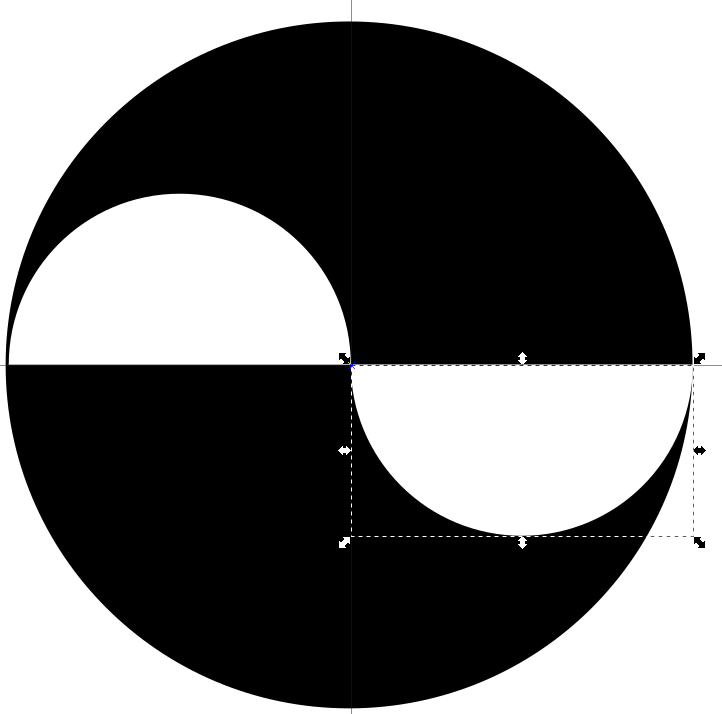
\includegraphics[width=1\linewidth]{5_6_moving.png}}\\
        Перемещение фигур
    \end{minipage}
    \vspace*{1cm}
    \vfill
    \begin{minipage}[h]{0.47\linewidth}
        \center{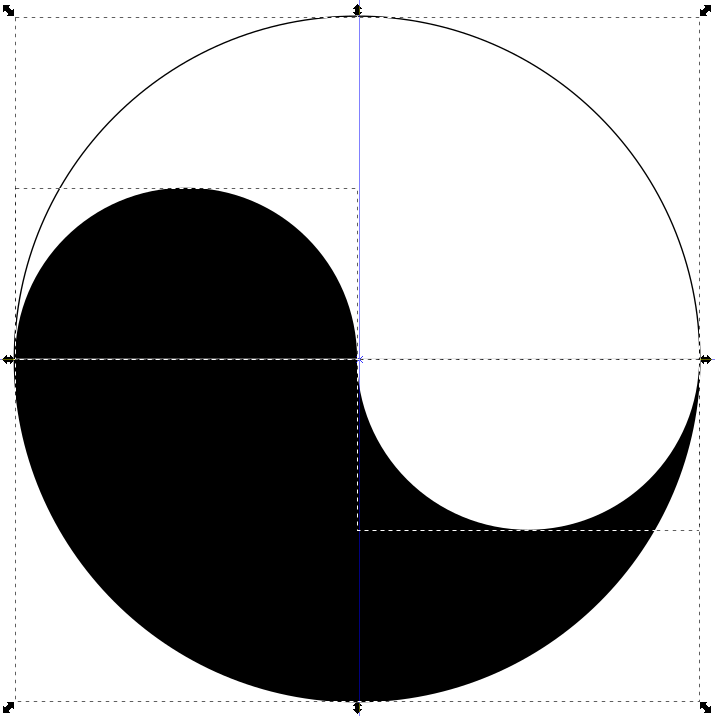
\includegraphics[width=1\linewidth]{5_7_color_change}}\\
        Изменение цветов заливки
    \end{minipage}
    \hfill
    \begin{minipage}[h]{0.47\linewidth}
        \center{
\includegraphics[width=1\linewidth]{5_8_circles_create.png}}\\
        Создание дополнительных фигур. Удаление вспомагательных линий
    \end{minipage}
\end{figure}
